\documentclass{beamer}
%%%%%%%%%%%%%%%%%%%%%%%%%%%%%%%  Packages  %%%%%%%%%%%%%
\usepackage{amsmath} 
\usepackage{mathtools}
\usepackage{physics}
\usepackage{amssymb}
\usepackage{mathptmx}
\usepackage{array}
  
%%%%%%%%% FIGurES %%%%%%%%%%%%%%%%%%%%%%%%
\usepackage{textcomp}
\usepackage{graphicx}
\usepackage{caption} 
\usepackage{subcaption}
\usepackage{scrextend}
\usepackage{rotating}
\usepackage{float}
\usepackage{hyperref}
\graphicspath{{./figures/}}
\hypersetup{colorlinks=true, citecolor=blue, linkcolor=blue}
\renewcommand{\equationautorefname}{Eq.}
\renewcommand{\figureautorefname}{Fig.}
 
%%%%%%%%%%%% LaNgUaGe %%%%%%%%%%%%%%%%%%
\usepackage{verbatim}
\usepackage{natbib}
\usepackage{wrapfig}

\usepackage[utf8]{inputenc}
\usetheme{PaloAlto}

\title{Modelling Nonlinear optics with the Bloch-Messiah reduction}
\author{Oliver Thomas}
\institute{Quantum Engineering CDT \\ University of Bristol}
\date{\today}

% plan

\begin{document}

\frame{\titlepage}

% slide 1
\begin{frame}
\frametitle{Why you should use version control}
\begin{itemize}
	\item What is nonlinear optics?
    \item Why do we care about it?
    \item  
\end{itemize}
\begin{figure}[H]
	\centering
	
\includegraphics[width=0.26\textwidth]{xkcdversion.png}
	\caption{Integrated optical chip with 16 single photon sources }
    \label{fig:big chip}
\end{figure}
\end{frame}

%slide 2
\begin{frame}
\frametitle{What is Git?}
\begin{itemize}
\item Git is one of most used version control software in the world 
\item Git is cross-platform and easy to use \footnotemark.
\end{itemize}
\footnotetext[2]{\url{https://try.github.io/levels/1/challenges/1}}
\end{frame}

%slide 2
\begin{frame}
\frametitle{What is GitHub?}
\begin{itemize} 
\item Github is a cloud service for git which lets you store your repository online
\item Why would you store your repository online?
\begin{itemize}
\item Working remotely
\item Collaborative work  
\item Hard drive failure!
\end{itemize}
\end{itemize}
\end{frame}


%slide 3
\begin{frame}
\frametitle{Making a repository}
\begin{itemize}
\item You can do this online on the Github website \footnotemark  
\item Create a new repository
\item Then click clone to get the url, open git on your computer and type: \\ 
	\texttt{git clone url}
\end{itemize}
\footnotetext[3]{\url{https://github.com/}}
\end{frame}

%slide 3
\begin{frame}
\frametitle{Making a repository}
\begin{itemize}
	\item Go to the folder and right click \texttt{git with bash}
\item You are now able to use bash for the rest of the talk!
\end{itemize}
\end{frame}

%slide 4
\begin{frame}
\frametitle{Basic Git commands}
\begin{itemize}
	\item There are four\footnotemark\ important commands you will need for git:
	\item \texttt{git pull}
	\item \texttt{git add *}
	\item \texttt{git commit -a}
	\item \texttt{git push}
\end{itemize}
\footnotetext[1]{I cheat here and write a bash script which does these in order so I only have to run a single command.}
\end{frame}

%slide 4
\begin{frame}
\frametitle{Advanced Git commands}
\begin{itemize}
	\item One of the great things about Git is that you can get by with just the four above commands.
	\item The git man page is very useful, especially, \\
	\texttt{man gittutorial} \\
	\texttt{man giteveryday} \\ 
\item \texttt{giteveryday} is a super useful collection of the 20 commands you will need regularly.
\end{itemize}
\end{frame}

%slide 4
\begin{frame}
\frametitle{Adding Collaborators}
\begin{itemize}
	\item Go to a repository and on the settings tab click collaborators, you can then search for the github username
\end{itemize}
\end{frame}



%slide 5
\begin{frame}
\frametitle{Why Python?} 
\begin{itemize}
	\item Python is popular, multi-platform and becoming a standard language\footnotemark\ 
	\item It is a good high level language to know, it is a very flexible interpreted language.
\end{itemize}
\footnotetext[2]{standard on most of the popular linux distributions}
\end{frame}

%slide 5
\begin{frame}
\frametitle{Python syntax} 
\begin{itemize}
	\item As with every programming language we should figure out how to do \textit{Hello, world!}
\end{itemize}
Open python and type:
\begin{verbatim}
print 'Hello, world!'
\end{verbatim}
\begin{itemize}
\item As Python is an interpreted language you can run command by command in python or use an IDE and then use python to run the program. For plotting it is more useful to write the program out in an IDE first. 
\end{itemize}
\end{frame}

%slide 2
\begin{frame}
	\frametitle{Adding your first commit}
\begin{itemize}
	\item Save your \textit{hello, world!} program. 
	\item Then either run: 
	\item \texttt{git add *}
	\item \texttt{git commit -a}
	\item \texttt{git push}
\end{itemize}

Or use the windows GUI version and commit them to your repository.
\end{frame}


%slide 6
\begin{frame}
\frametitle{Plotting}
\begin{itemize}
	\item Python requires the \texttt{numpy} library\footnotemark\ for a lot of basic maths functions (and arrays).
	\item We are going to use the \texttt{matplotlib} library\footnotemark\ for the remainder of this talk. 
\end{itemize}
\footnotetext[3]{\url{http://www.numpy.org/}}
\footnotetext[4]{\url{https://matplotlib.org/api/_as_gen/matplotlib.pyplot.plot.html}}
\end{frame}

%slide 2
\begin{frame}
\frametitle{Example 1, Plotting functions}
\begin{itemize}
	\item Go to the \texttt{src} folder and open \texttt{ex1functions.py} 
	\item Run \texttt{all.py} and choose 1 
\end{itemize}
\end{frame}

%slide 2
\begin{frame}
\frametitle{Example 1, Plotting functions}
\begin{figure}
	\centering
	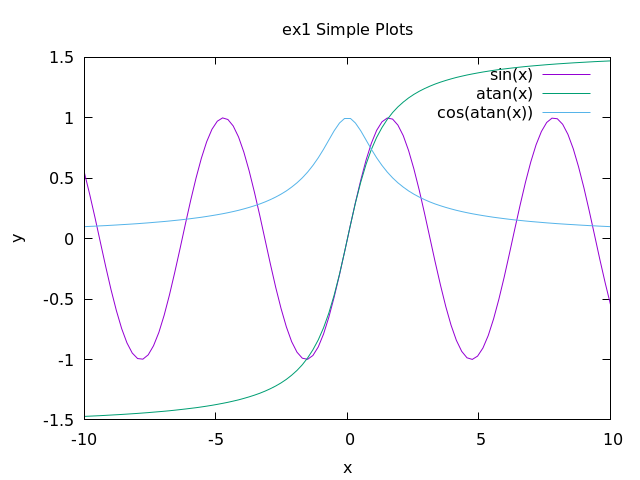
\includegraphics[width=0.5\textwidth]{ex1.png}
	\caption{function plotting}
	\label{fig:function}
\end{figure}
\begin{itemize}
	\item It could do with some axis labels. 
	\item go into the program and find the line called \texttt{plt.ylabel=} and \texttt{plt.xlabel=}  
\end{itemize}
\end{frame}

%slide 2
\begin{frame}
\frametitle{Example 2, Complicated functions!}
\begin{itemize}
\item In the \texttt{src} folder open \texttt{ex2compfunctions.py} 
\item Run all.py and choose 2 
\end{itemize}
\end{frame}

%slide 2
\begin{frame}
\frametitle{Example 2, Complicated functions!}
\begin{itemize}
\item Figures!
\item
\end{itemize}
\begin{figure}
	\centering
	\includegraphics[width=0.5\textwidth]{aex2.png}
	\caption{function plotting}
	\label{fig:function}
\end{figure}
\end{frame}


%slide 2
\begin{frame}
\frametitle{Example 3, Plotting data!}
\begin{itemize}
	\item once again, in the \texttt{src} folder open \texttt{ex3data.py}
	\item Run all.py and choose 3 
\end{itemize}
\end{frame}

%slide 2
\begin{frame}
\frametitle{Example 3, Plotting data!}
\begin{itemize}
	\item figure 
\end{itemize}
\begin{figure}
	\centering
	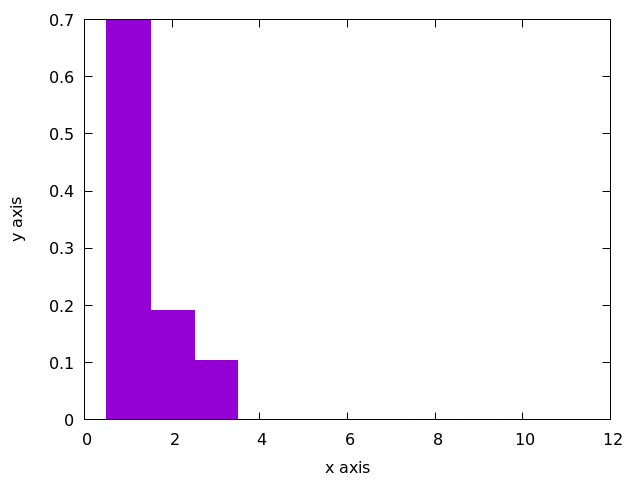
\includegraphics[width=0.5\textwidth]{ex3.png}
	\caption{function plotting}
	\label{fig:function}
\end{figure}
\end{frame}

%slide 2
\begin{frame}
\frametitle{Example 4, Histograms!}
\begin{itemize}
\item once again, in the \texttt{src} folder open \texttt{ex4hist.py}
	\item Run all.py and choose 4 
\end{itemize}
\end{frame}

%slide 2
\begin{frame}
\frametitle{Example 4, Histograms!}
\begin{itemize}
\item figure
\end{itemize}
\begin{figure}
	\centering
	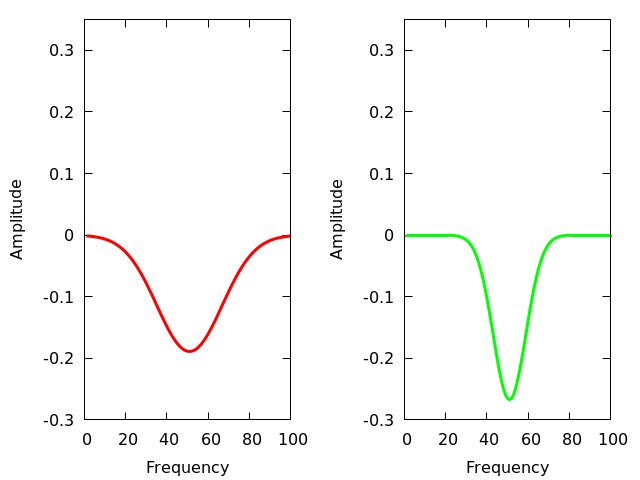
\includegraphics[width=0.5\textwidth]{ex4.png}
	\caption{function plotting}
	\label{fig:function}
\end{figure}
\end{frame}

%slide 2
\begin{frame}
\frametitle{Example 5, Subplots!}
\begin{itemize}
\item In the \texttt{src} folder open \texttt{ex5subplots.py} 
	\item Run all.py and choose 5 
\end{itemize}
\end{frame}

%slide 2
\begin{frame}
\frametitle{Example 5, Subplots!}
\begin{itemize}
\item Figures!
\end{itemize}
\begin{figure}
	\centering
	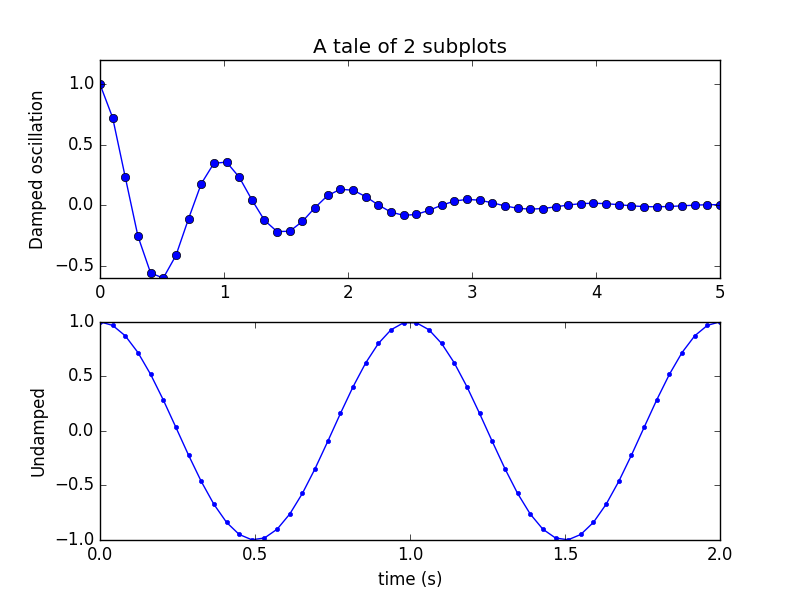
\includegraphics[width=0.5\textwidth]{ex5.png}
	\caption{function plotting}
	\label{fig:function}
\end{figure}
\end{frame}

%slide 2
\begin{frame}
\frametitle{Example 6, Art!}
\begin{itemize}
\item In the \texttt{src} folder open \texttt{ex6art.py} 
	\item Run all.py and choose 6 
\end{itemize}
\end{frame}

%slide 2
\begin{frame}
\frametitle{Example 6, Art!}
\begin{itemize}
\item Figures!
\end{itemize}
\begin{figure}
	\centering
	\includegraphics[width=0.5\textwidth]{aex6.png}
	\caption{function plotting}
	\label{fig:function}
\end{figure}
\end{frame}

%slide 2
\begin{frame}
\frametitle{Branching}
\begin{itemize}
\item Branching is useful, it lets you test something out separately to the main branch.
\item To make a new branch called \texttt{test} \\
\texttt{git branch test} 
\item You can check all of the current branches and which branch you are on with \\
	\texttt{git branch}
\end{itemize}
\end{frame}

%slide 2
\begin{frame}
\frametitle{Branching}
\begin{itemize}
	\item To switch to the test branch type: \\ 
	\texttt{git checkout test} \\
\end{itemize}
\end{frame}

%slide 2
\begin{frame}
\frametitle{Thanks for listening!}
\begin{figure}[H]
	\centering
	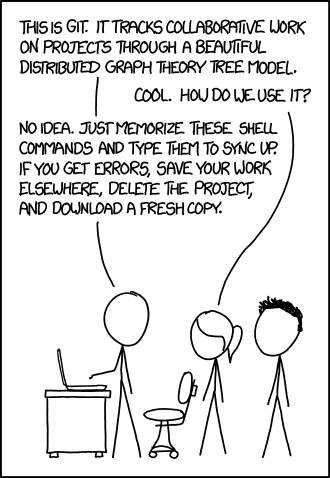
\includegraphics[width=0.4\textwidth]{xkcdgit.png}
	\caption{If it all goes wrong \ldots \footnotemark }
	\label{fig:xkcdversion}
\end{figure}
\footnotetext[1]{\url{https://xkcd.com/1597/}}
\end{frame}











\end{document}
